\chapter{Methodology}\label{chap:methodology}

In this chapter, we will detail the pillar of our proposed methodology for our end-to-end framework that aims to find the optimal bit-width for each layer of QNN while ensuring that the defined bit-widths satisfy robustness properties using the SMT Theory of Fixed-Point Arithmetic.

%replaced by below
%This work is based on Cai et al.'s framework called Quadapter \cite{cai2025certified}, a framework for synthesizing QNN that are robust against adversarial attack using MILP solvers. However, unlike Quadapter, which relies on idealized mathematical models, our approach aims to incorporate the SMT Theory of Fixed-Point Arithmetic to ensure that the synthesized QNNs are verified under finite-precision arithmetic.

%Our work is based on Cai et al.'s Quadapter \cite{cai2025certified}, which synthesizes a QNN from a regular floating-point precision ANN to keep it robust against adversarial attacks by using MILP solver to verify for vulnerabilties and thus use the information to find the best bit-width for quantization. However, unlike his work, ours aims to incorporate the SMT Theory of verifying Fixed-point arithmetic to ensure that the found QNN is also verified under finite-precision arithmetic.
Our work is built upon Cai et al.'s Quadapter \cite{cai2025certified}, which aims to convert a traditional floating-point Neural Network into a similar fixed-point QNN with an enhanced robustness against adversarial attacks within the quantized model. This is achieved by employing an MILP solver to identify vulnerabilities and determine the optimal quantization bit-width for each layer. In contrast, our approach integrates an SMT solver to verify the defined constraints, accounting for the particulars of fixed-point arithmetic, thereby ensuring that the resulting QNN is rigorously validated under finite-precision arithmetic constraints \cite{baranowski2020smt}.

%Similarly, Quadapter, our framework, also computes the preimage of each ANN layer and uses it to define the optimal bit-width for each layer $\xi_{i}$, while ensuring that the robustness property is satisfied. The safety property will be verified using an off-the-shelf SMT-based verifier, such as ESBMC \cite{esbmc2025}, that supports fixed-point arithmetic.
Similarly to Quadapter, our framework, also computes the preimage of each ANN layer and uses it to define the optimal bit-width for each layer $\xi_{i}$ by selecting the best set that ensures the robustness property is satisfied. The safety property is verified using an off-the-shelf SMT-based verifier, ESBMC \cite{esbmc2025}, that supports fixed-point arithmetic.

The general methodology of our proposed framework is summarized in the diagram shown in Figure \ref{fig:diagrama_metodologia} and detailed in the Algorithm \ref{alg:quantization_synthesis}.

\newpage
\begin{comment}
    
\begin{figure}[!hb]
\centering
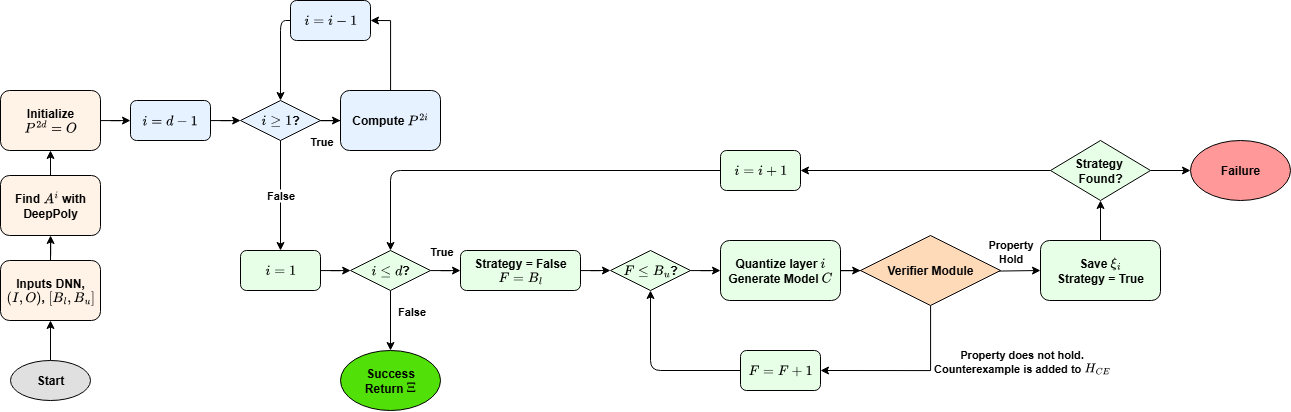
\includegraphics[width=1\textwidth]{figuras/3-metodologia/diagram_v1.png
}
\caption{Proposed Methodology Diagram}
\label{fig:diagrama_metodologia}
\end{figure}
\end{comment}

\begin{figure}[!hb]
\centering
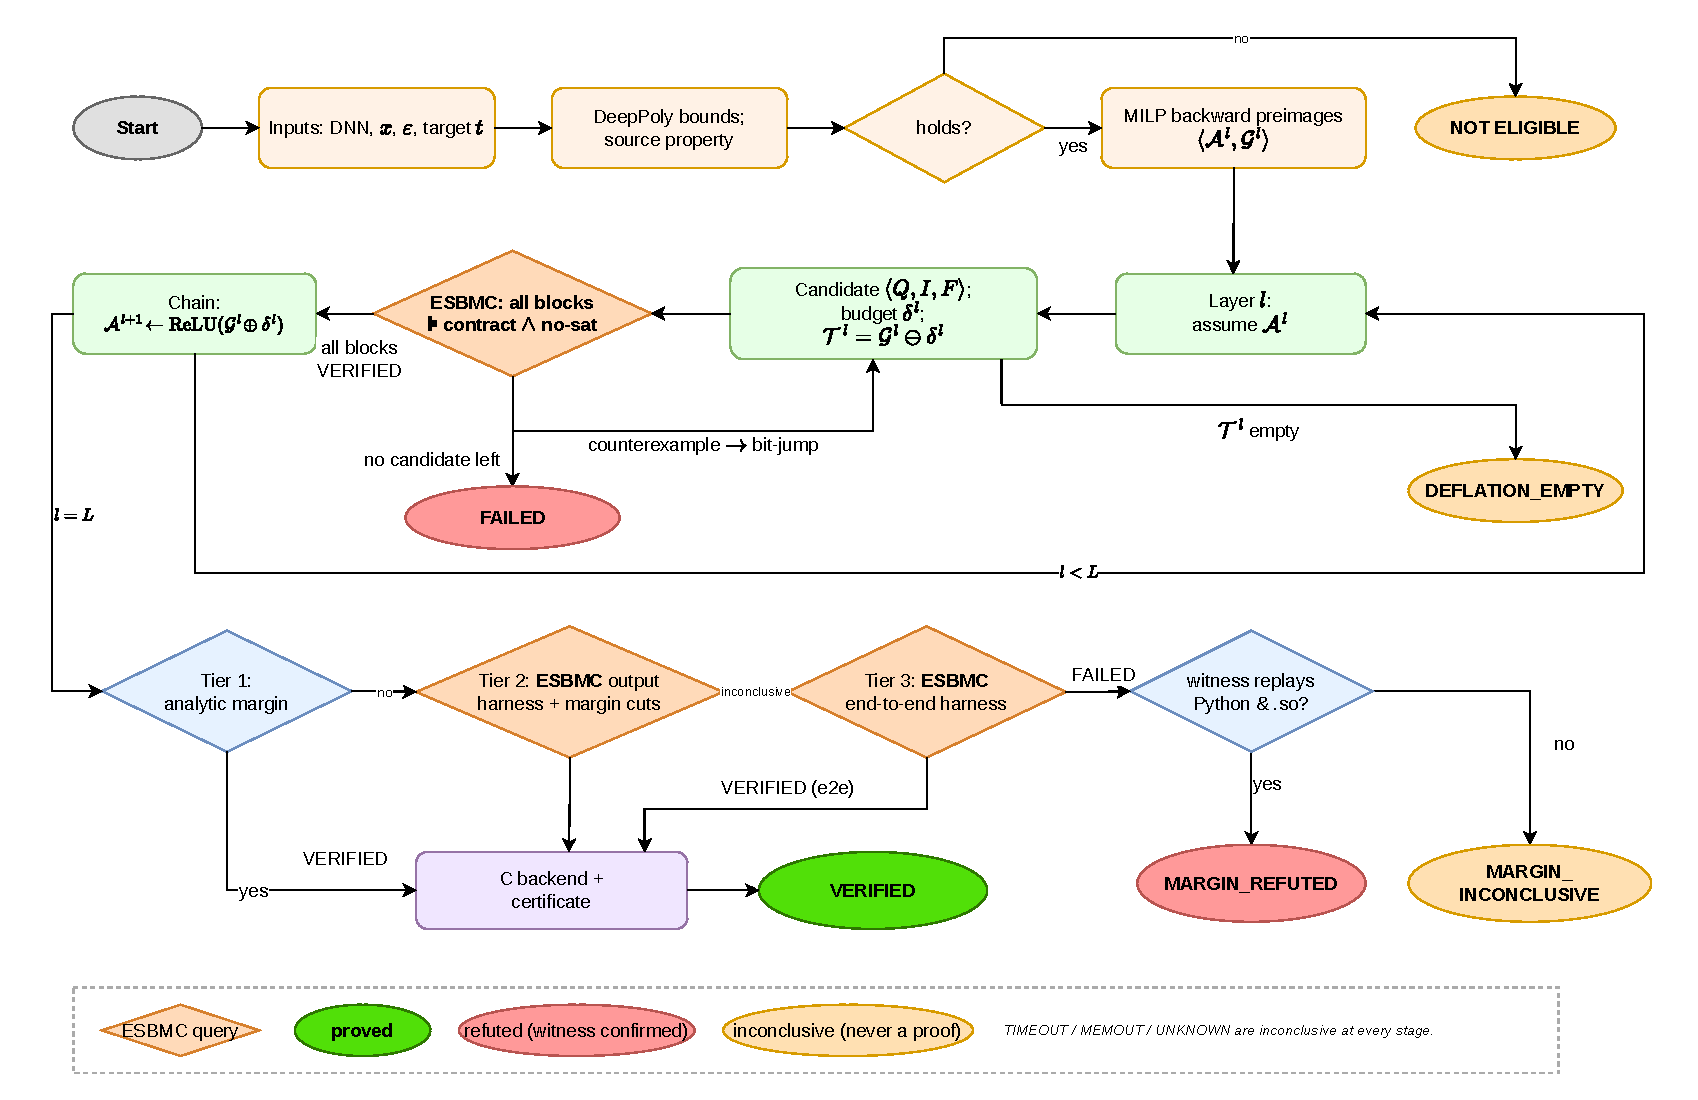
\includegraphics[width=1\textwidth]{figuras/3-metodologia/main_diagram_preqbmc_pdf.drawio.pdf}


\caption{Proposed Methodology Diagram}
\label{fig:diagrama_metodologia}

\end{figure}

%We call the original ANN as $\mathcal{N}$ and the quantized neural network as ${\hat{\mathcal N}}$. The layers of the ANN are represented as $f_i$ and the layers of the QNN as $\hat{f_i}$. The preimage of each layer $f_i$ is represented as $P_i$ and it represents the under-approximation $P^{2l} \subseteq \mathcal N^{1:2i}_{2i}(\mathcal O)$. Our approach decomposes this global verification problem into a series of layer-wise counter-example verification problems. Specifically, for each affine layer $f_{2i}$. Initially, we use the DeepPoly \cite{singhAbstractDomainCertifying2019} abstract interpretation framework to prove that the original floating-point DNN satisfies the robustness property and to compute admissible output intervals for each layer, $\mathcal{A}^i_{j}$. Next, we perform a backward preimage computation to derive output intervals for each layer that are sufficient to guarantee the overall robustness property. These intervals are defined by $P^{2l}$ and will be used to guide the synthesis of the QNN. Then, for each layer independently, we verify that its quantized counterpart $\hat{f_{2i}}$ satisfies the property shown in Equation \ref{eq:main_preposition_milp} which ensures that the quantized affine layer's output falls within the calculated preimage, thus implying that the entire quantized network $\hat{N}$ satisfies the global robustness property defined.
We call the original ANN as $\mathcal{N}$ and the quantized neural network as ${\hat{\mathcal N}}$. The layers of the ANN are represented as $f^{[l]}$ and the layers of the QNN as $\hat{f^{[l]}}$. The preimage of each layer $f^{[l]}$ is represented as $P_i$ and it represents the under-approximation $P^{2[l]} \subseteq \mathcal N^{1:2[l]}_{2[l]}(\mathcal O)$. Our approach decomposes this global verification problem into a series of layer-wise counter-example verification problems. Specifically, for each affine layer $f^{2[l]}$. Initially, we use the DeepPoly \cite{singhAbstractDomainCertifying2019} abstract interpretation framework to prove that the original floating-point ANN satisfies the robustness property and to compute admissible output intervals for each layer, $\mathcal{A}^{[l]}_{j}$. Next, we perform a backward preimage computation to derive output intervals for each layer that are sufficient to guarantee the overall robustness property. These intervals are defined by $P^{2[l]}$ and will be used to guide the synthesis of the QNN. For each affine quantized layer, $\hat{f^{2[l]}}$, we verify whether the condition in equation \ref{eq:main_preposition_milp} holds. By confirming this property at every layer, we establish that the entire $\mathcal{ \hat{N}}$ satisfies the global robustness property.


\begin{equation}\label{eq:main_preposition_milp}
    %\hat{N}^{1:2[l]}_{2[l]}(\mathcal I) \subseteq P^{2[l]} \implies \hat{N} \vDash <\mathcal I, \mathcal O>
\hat{\mathcal{N}}^{1:2[l]}_{2[l]}(\mathcal{I}) \subseteq P^{2[l]} \implies \hat{\mathcal{N}} \models \langle \mathcal{I}, \mathcal{O} \rangle
\end{equation}

%% Algorithm
\begin{algorithm}[H]
\caption{SMT-Based Quantization Synthesis for Robust Neural Networks}
\label{alg:quantization_synthesis}
\begin{algorithmic}[1]
\Require Original network $\mathcal N$, input region $\mathcal{I}$, output region $\mathcal{O}$, bit-width search space $\Xi$
\Ensure Quantized network $\mathcal{\hat{N}}$ satisfying robustness property, or synthesis failure
\State \textbf{Phase 1:} Compute $\mathcal{A}^{[l]}_{j}$ using DeepPoly and backward preimage $P^{2l}$ from $\mathcal{O}$
\For{each affine layer $f^{2[l]} \in \mathcal N$}
    \For{each bit-width configuration $\xi_{[l]} \in \Xi$}
        \State Quantize $\mathbf{W}^{2[l]}, \mathbf{b}_{2l}$ with $\xi_{[l]} = \langle Q_{[l]}, F_{[l]} \rangle$
        \State Generate C harness for $\hat{f}^{2[l]}$ with fixed-point arithmetic
        \State Encode constraint $\mathcal{\hat{N}}^{1:2[l]}_{2[l]}(\mathcal{I}) \subseteq P^{2[l]}$ as SMT assertions
        \State $\text{result} \gets$ \Call{ESBMC-Verify}{C harness, timeout}
        \If{$\text{result} = \textsc{Verified}$}
            \State Record $\xi_{[l]}^* \gets \xi_{[l]}$ and \textbf{break}
        \EndIf
    \EndFor
    \If{no verified configuration found}
        \State \Return \textsc{Synthesis-Failure} for layer $[l]$
    \EndIf
\EndFor
\State \textbf{return} $\hat{N}$ with $\Xi = \{\xi_1^*, \xi_2^*, \ldots, \xi_d^*\}$
\end{algorithmic}
\end{algorithm}

\section{Input Region Definition and Initialization}
% Text below had indices of AI usage. We will fix it.
%The verification process begins by defining the input uncertainty region in the main entry point of the program. Given the input $x$ $\forall$ $\in$ $\mathbb{R}^n$ and the pertubation $\delta$ such that $||\delta||_\infty \leq \epsilon$, we define the input bounds as follows: $x_{low} = clip(x - \epsilon)$ and $x_{high} = clip( x + \epsilon)$, where the clip function ensures that the extubated inputs remain within the valid input range domain. For datasets like iris and seeds, the dataset perturbation is determined by the natural features of the data. \textcolor{blue}{For example for the iris dataset or seeds one the addition of $\epsilon$ could not make sense, as $0.01$ could not be enough to be considered a significant perturbation. Thus, for these datasets, we define a normalized perturbation based on the standard deviation of each feature in the dataset.}



The verification procedure starts by defining an uncertainty region around the input at the program's main entry point. Let $x \in \mathbb{R}^n$ be the nominal input and let $\delta$ be a perturbation such that $\lVert \delta \rVert_\infty \leq \epsilon$. From this, we obtain lower and upper bounds for the input:
\begin{equation}
    x_{\text{low}} = \operatorname{clip}(x - \epsilon),
    \qquad
    x_{\text{high}} = \operatorname{clip}(x + \epsilon),
\end{equation}
where the function $\operatorname{clip}(\cdot)$ keeps each feature inside its valid range.

For image-like data, using a fixed $\epsilon$ in the original scale is usually reasonable, because all features share a similar range. For tabular data, however, this is not always the case. In datasets such as \textit{Iris} or \textit{Seeds}, different features can have very different scales, so a small value like $\epsilon = 0.01$ may be almost irrelevant for some features and too strong for others. To avoid this issue, we use a feature-wise normalized perturbation based on each feature's standard deviation. For each feature $j$, we define
\begin{equation}
    \epsilon_j = \kappa \sigma_j,
\end{equation}
where $\sigma_j$ is the standard deviation of feature $j$ in the dataset and $\kappa$ is a user-defined factor that controls the size of the perturbation. The bounds are then computed as
\begin{equation}
    x_{\text{low}} = \operatorname{clip}(x - \epsilon_j),
    \qquad
    x_{\text{high}} = \operatorname{clip}(x + \epsilon_j),
\end{equation}
with $\epsilon = (\epsilon_1, \dots, \epsilon_n)$.


\begin{comment}
    As explained in the paragraph before, the use of just a variable does not make sense as for some dataset the variable may influence a lot bot for other it may just be a insignificant change. Thus, we have some options as below:
        - Make the normalization based on the standard deviation of each feature in the dataset.

\end{comment}

\section{Symbolic Bound Propagation}
%With the input region defined by $\mathcal{I}$, the DeepPoly abstract interpretation framework is instantiated to compute the concrete lower and upper bounds for every neural of ANN. It performs a forward pass through the network, maintaining  symbolic linear constraints that express each neuron's activation as a function of the input variables like shown in Figure \ref{fig:preimage_backpropagation}. For each affine layer transformation, DeepPoly computes both concrete bounds and symbolic bounds and the symbolic constraints that relate the output to the input.

%The results of this propagation are stored in the layer structures of the network. For each $f_i$, the framework maintain several sets of bounds: $l_i$ and $u_i$ represent respectively the concrete lower and upper bounds of the affine $i$ layer outputs.
With the input region defined by $\mathcal{I}$, the DeepPoly abstract interpretation framework is instantiated to compute the concrete lower and upper bounds for every neural network of ANN. It performs a forward pass through the network, maintaining  symbolic linear constraints that express each neuron's activation as a function of the input variables, as shown in Figure \ref{fig:preimage_backpropagation}. For each affine-layer transformation, DeepPoly computes both concrete and symbolic bounds, as well as the symbolic constraints relating the output to the input.

The results of this propagation are stored in the network's layer structures. For each $f^{[l]}$, the framework maintains several sets of bounds: $l_i$ and $u_i$ represent the concrete lower and upper bounds of the affine $i$ layer outputs.

\section{Backward Preimage Computation}
%The backward image computation is crucial for decomposing the global verification problem into a layer-wise sub-problem. By knowing the desired output region $\mathcal{O}$ of output layer, we compute the under-approximation of the preimage $P^{2d}$ for each affine layer $f^{2i}$. This preimage represents the set of output domain of each layer, thus by knowing that the output of last layer is $\mathcal{O}$, we can compute the preimage of the last affine layer $P^{2d}$ and then use it to compute the preimage of the previous layer $P^{2(d-1)}$ and so on until reaching the first layer $P^{0}$. The preimage is also computed to the activation layers by propagating the preimage through the activation functions to later use it in the verification of the next affine layer.

%This backward propagation is conservative in the sense that the computed preimages may be smaller than strictly necessary, but it guarantees that if the quantized layer's output falls within this preimage, then all the subsequent layers will also behave correctly. This conservatism is essential for ensuring the soundness of the layer-wise verification approach \textcolor{red}{WHY???}. The preimage intervals serve as the verification targets during the subsequent ESBMC verification step for each quantized layer.
The backward image computation is crucial for decomposing the global verification problem into a layer-wise sub-problem. By knowing the desired output region $\mathcal{O}$ of the output layer, we compute the under-approximation of the preimage $P^{2d}$ for each affine layer $f^{2[l]}$. This preimage represents the set of output domain of each layer, thus by knowing that the output of last layer is $\mathcal{O}$, we can compute the preimage of the last affine layer $P^{2d}$ and then use it to compute the preimage of the previous layer $P^{2(d-1)}$ and so on until reaching the first layer $P^{0}$. The preimage is also computed for the activation layers by propagating it through the activation functions for later use in verifying the next affine layer.

The mentioned backward calculation of the preimage is conservative, i.e., an underapproximation of the real region; thus, it may represent a smaller region than strictly necessary, but it guarantees that if the quantized layer is within its bounds, all subsequent layers will also behave correctly. The preimage intervals serve as the verification targets during the subsequent ESBMC verification step for each quantized layer.
\begin{figure}[!hb]
\centering
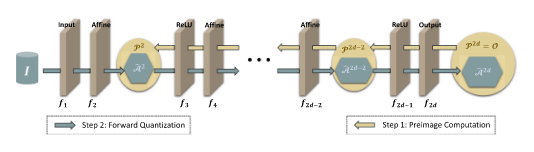
\includegraphics[width=0.8\textwidth]{figuras/3-metodologia/preimage_backpropagation.png} 
\caption{Backpropagation of Preimage through the Network Layers \cite{cai2025certified}}
\label{fig:preimage_backpropagation}
\end{figure}

\section{Quantization Search with ESBMC}
\begin{comment}
    
$The method implements the core quantization verification loop, systematically searching for the optimal bit-width configuration $\mathcal <Q, F\mathcal>$ where  $Q$ is the total bit-width and $F$ is the number of fractional bits for each layer that ensures the satisfaction of the robustness property.  The method iterates over each affine layer of the network until reach the output, and for each layer, it explores a range of bit-width, the method tries different divisions between integer and fractional bits to find the optimal configuration. Once found the configuration $\xi _{i}$ for layer $i$, it is fixed and the method proceeds to the next layer. The set of possible solutions is defined as $\varXi = {\{\xi _1, \xi _2, ..., \xi _{d}\}}$ where $d$ is the number of layers. 

$For a given configuration, the layer's weight and biases are quantized by scaling them by $2^{fractional\_bits}$ and rounding to the nearest integer: $round(weight * 2^{fractional\_bits})$ and $round(bias * 2^{fractional\_bits})$. This quantization scheme represents values in QF format, where arithmetic operation are performed on integers that implicitly represent fixed-point numbers with $F$ fractional bits. 

$The search strategy is greedy as for each layer the method tries bit-widths from the smallest to largest, and for each bit-width, it tries configurations with different fractional bit allocations. As soon as ESBMC successfully verifies a passing configuration, the method records this configuration and moves to the next layer. If no configuration passes for a given layer, the method raises an exception indicating that the quantization synthesis has failed for the network.
\end{comment}

The method implements the core quantization verification loop, systematically searching for the optimal bit-width configuration $\mathcal <Q, F\mathcal>$ where  $Q$ is the total bit-width and $F$ is the number of fractional bits per layer that ensures the satisfaction of the robustness property.  The method iterates over each affine layer of the network until it reaches the output, and for each layer, it explores a range of bit-width. The method tries different divisions between integer and fractional bits to find the optimal configuration. Once found, the configuration $\xi _{[l]}$ for layer $i$ it is fixed, and the method proceeds to the next layer. The set of possible solutions is defined as $\varXi = {\{\xi _1, \xi _2, ..., \xi _{d}\}}$ where $d$ is the number of layers. 

For a given configuration, the layer's weight and biases are quantized by scaling them by $2^{fractional\_bits}$ and rounding to the nearest integer: $round(weight * 2^{fractional\_bits})$ and $round(bias * 2^{fractional\_bits})$. This quantization scheme represents values in QF format, where arithmetic operations are performed on integers that implicitly represent fixed-point numbers with $F$ fractional bits. 

The search strategy is greedy: for each layer, the method tries bit-widths from the smallest to largest, and for each bit-width, it tries configurations with different fractional bit allocations. As soon as ESBMC successfully verifies a passing configuration, it records the configuration and proceeds to the next layer. If no configuration passes for a given layer, the method throws an exception indicating that the quantization synthesis has failed for the network.

\subsection{QNN Code Generation}
\begin{comment}
    - Usually ANN are thought as mathematical functions, but in reality they are implemented in HW as source code of a certain language. Thus, we can think it as a code verification problem.
    - We use C Language as an abstraction of QNN implementation
\end{comment}
%In the Machine Learning community, ANNs are typically represented as mathematical functions that map the input space to the outer space through a series of layers and activation functions. Our work, rather than focusing on the mathematical representation of ANNs, adopts a code-centric perspective, viewing ANNs as programs implemented in a C programming language. Thus, we approach the verification of the ANNs as a code verification problem like proposed by other works such as Cordeiro et al. \cite{cordeiro2025neuralnetworkverificationprogramming} and Sena et al. \cite{abdi2021counterexample}.
In the Machine Learning community, ANNs are typically represented as mathematical functions that map the input space to the outer space through a series of layers and activation functions. Our work, rather than focusing on the mathematical representation of ANNs, adopts a code-centric perspective, treating ANNs as programs implemented in the C programming language. Thus, we approach the verification of the ANNs as a code verification problem, as proposed by other works as Sena et al. \cite{abdi2021counterexample} and subsequently Cordeiro et al. \cite{cordeiro2025neuralnetworkverificationprogramming}.
\subsection{Introducing Safety Properties in ANN Code}\label{sec:safety_prop}

%As described before, we intend to use the SMT Theory to verify safety properties in QNNs. To do so, we will follow the approach proposed by Cordeiro et al. \cite{cordeiro2025neuralnetworkverificationprogramming} that consists of translating the neural network and the safety property into a C program. This program can then be verified using an SMT-based verifier like ESBMC \cite{esbmc2025}.

%Since the Bound Model Check technique used by ESBMC explores all possible execution paths of the program up to a certain depth, it was necessary to make use of non-deterministic variables to represent the inputs of the neural network. This allows ESBMC to explore all possible input combinations and verify if the safety property holds to all possible inputs. Thus, the first step in our methodology is to define the input variables of the neural network as non-deterministic variables in the C code. This can be done using the following notation:
As described before, we intend to use the SMT Theory to verify safety properties in QNNs. To do so, we follow the approach proposed by Cordeiro et al. \cite{cordeiro2025neuralnetworkverificationprogramming} that consists of translating the neural network and the safety property into a C program. This program can then be verified using an SMT-based verifier like ESBMC \cite{esbmc2025}.

Since the Bound Model Check technique used by ESBMC explores all possible execution paths of the program up to a given k-depth, it was necessary to use nondeterministic variables to represent the neural network’s input. This allows ESBMC to explore all possible input combinations and verify if the safety property holds for an n-set of possible inputs. Thus, the first step in our methodology is to define the neural network's input variables as nondeterministic in the C code. This can be done using the following notation:
\begin{equation}
    \begin{aligned}
    \texttt{in\_[j] = nondet\_longlong();}
    \end{aligned}
\end{equation}

%Let's consider the robustness property as an example. To verify if a neural network is robust against adversarial attacks within a certain radius $\epsilon$ under the $\ell^\infty$ norm, we need to ensure that for any input $x$ and any perturbation $\delta$ such that $||\delta||_\infty \leq \epsilon$, the output of the neural network remains unchanged. Consequently, we encode the premise with precondition assertions that define the input space and the pertubation limits within the bound of the original ANN. \textcolor{red}{Explain the perturbation is already included in the input bounds}
To verify if a neural network is robust, we are considering a perturbation radius $\epsilon$ under the $\ell^\infty$ norm. In resume: we need to ensure that for any input $x$, and any perturbation $\delta$ such that $||\delta||_\infty \leq \epsilon$, the output of the QNN will remain unchanged. Consequently, we encode the premise as precondition assertions that define the input space and the perturbation limits within the original ANN's bounds. 
\begin{equation}
    \begin{aligned}
    \texttt{\_\_ESBMC\_assume(in\_[j] >= input\_bounds\_low[j] \&\&} \\
    \texttt{in\_[j] <= input\_bounds\_high[j]);}
    \end{aligned}
\end{equation}

This notation ensures that the SMT solver only considers input within the specified assumption bounds. Next, we need to encode the conclusion of the robustness property using post-condition assertions that check if the output of the neural network remains unchanged for all perturbed inputs within the defined bounds by checking for a counter-example, i.e., if there exists an output that falls outside the expected range defined by the preimage of the output layer.


\begin{equation}
    \begin{aligned}
    \texttt{\_\_ESBMC\_assert(s\_out >= pre\_lo - eps \&\& s\_out <= pre\_hi + eps)}
    \end{aligned}
\end{equation}
%%%%%%%%%%%%%%%%%%%%%%%%%%%%%%%%% STOPPED Verifing Here
In case of ESBMC finding a counter-example, i.e., an example that violates the defined assertion, it would indicate by the definition of the assertion that the QNN is not robust, thus the $\xi _{x}$ configuration is not safe, therefore it must dismiss that configuration and try with another one until no counter-example is found. Conversely, if no counter-example is found within the specified bounds, it confirms that the QNN maintains its robustness property under the defined perturbations. 

\section{ESBMC Execution}
The framework calls for the ESBMC instance tool version 7.11 to verify the safety property on the generated C harness and to interpret the results. ESBMC is invoked with a carefully chosen set of command-line options that balance verification power with execution time. 

\begin{itemize}
    \item \texttt{-{}-boolevectors} chooses the Boolevector solver as it shows better performance in previous works \cite{li2025esbmcv76enhancedmodel}.
    \item \texttt{-{}-ir} use of integral/real arithmetic for fixed-point operations verification.
    \item \texttt{-{}-loop-invariant} enables loop invariant generation, which can help ESBMC reason about loops more effectively.
    \item \texttt{--incremental-bmc} enables incremental bounded model checking, which can improve performance by reusing solver state across different unrolling depths.
    \item \texttt{-{}-interval-analysis} activates interval analysis to compute variable bounds, aiding in pruning infeasible paths.
    \item \texttt{--no-unwinding-assertions} disables unwinding assertions to reduce overhead when loops are fully unrolled.
    \item \texttt{-{}-state-hashing} enables state hashing to avoid redundant exploration of identical program states.
\end{itemize}

Among others, \texttt{-{}-no-bounds-check}, \texttt{-{}-no-div-by-zero-check}, and \texttt{-{}-no-pointer-check} to disable unnecessary checks that are not relevant for our verification task.

To report verification status, our verification module parses the ESBMC output to determine the verification outcome. The ESBMC has three predefined outputs; the first would be ``VERIFICATION SUCCESSFUL'' to indicate successful verification, i.e., no counter-example was found in the assertion verification; the second would be ``VERIFICATION FAILED'', i.e., a counter-example was found, indicating that the quantization of that layer for a specific bit-width is not robust; If neither success nor failure is reported, or if the tool runs out, the result is classified as `UNKNOWN'', and the method proceeds to try the next quantization configuration.

%The overall methodology provide formal soundness guarantees through the composition of sound techniques. DeepPoly's over-approximation ensures that the computed bound may include unreachable values. The backward preimage computation maintains this conservatism, computing for each layer a set of admissible outputs that is sufficient to guarantee correct final outputs. ESBMC's bounded model checking provides complete verification within the specified bounds and unrolling depth: if ESBMC reports success, then the quantized arithmetic provably satisfies the assertions for all inputs in the range.

%Therefore, the composition of these techniques ensure the preservation of sounds: if every hidden layer's quantized affine outputs fall within their respective preimages bound and if the output layer satisfies the argmax property, then the complete quantized network satisfies the global robustness property under finite-precision arithmetic.
The composition of these techniques and the use of SMT backend by ESBMC ensures the preservation of soundness within our methodology \cite{sena2021verifying}: if every hidden layer's quantized affine outputs fall within their respective preimages bound and if the output layer satisfies the argmax property, then the complete quantized network satisfies the global robustness property under finite-precision arithmetic.
\section{Central Problem}
%Several works in the literature have addressed the synthesis of QNNs that are robust against adversarial attacks. Notably, Cai et al. \cite{cai2025certified} introduced Quadapter, a framework that employs MILP solvers to synthesize quantized neural networks with certified robustness properties. However, a significant limitation of this approach is its reliance on idealized mathematical models that do not account for the intricacies of finite-precision arithmetic used in real-world implementations of QNNs. This discrepancy can lead to a behavioral gap between the synthesized model and its actual implementation, potentially undermining the robustness guarantees provided by the synthesis process.



The scope of our work is to construct a synthesis of QNNs that takes into consideration the safety property of robustness, and also is bit-precise with Integer Arithmetic. Cai et al. \cite{cai2025certified} introduced Quadapter, a framework that uses MILP solvers to synthesize quantized neural networks with certified robustness. However, a significant limitation of this approach is that it does not account for the bit precision of the matter; it treats quantization as a mathematical problem rather than a code problem, and thus it can lead to the omission of integer arithmetic in the quantization process. This discrepancy is addressed in our work by using SMT verifiers as a backend instead of MILP solvers, as reported by \cite{baranowski2020smt}. SMT verifiers are bit-precise and sound and can handle Integer arithmetic used in embedded hardware.


\section{Algortihm}

\newcommand{\fmt}[1]{\ensuremath{\langle n^{[#1]}, i^{[#1]}, f^{[#1]}\rangle}}
\newcommand{\Abox}[1]{\ensuremath{\mathcal{A}^{[#1]}}}
\newcommand{\Gbox}[1]{\ensuremath{\mathcal{G}^{[#1]}}}
\newcommand{\dbud}[1]{\ensuremath{\delta^{[#1]}}}
\newcommand{\Nfp}[1]{\ensuremath{\widehat{N}^{[#1]}_{\mathit{fp}}}}
\algrenewcommand\algorithmicrequire{\textbf{Input:}}
\algrenewcommand\algorithmicensure{\textbf{Output:}}


\begin{comment}
    
 
% =====================================================================
\begin{algorithm}[t]
\caption{PreQ-BMC: preimage-guided synthesis with derived error budgets}
\label{alg:preqbmc}
\small
\begin{algorithmic}[1]
\Require Trained network $N$ with layers $l=1,\dots,L$; sample $\mathbf{x}$;
         radius $\varepsilon$; target class $t$; bit range $[n_{lb},n_{ub}]$;
         block size $\beta$
\Ensure  Format $\Phi=\{\fmt{l}\}_{l=1}^{L}$, verdict, guarantee level
 
\Statex \textbf{\emph{Stage 1: contracts}}
\State $\Abox{1} \gets B_\varepsilon(\mathbf{x})$
\State $(\mathit{lb},\mathit{ub}) \gets \textsc{DeepPoly}(N, \Abox{1})$
   \Comment{sound forward bounds}
\For{$l = L$ \textbf{down to} $1$}
   \State $\Gbox{l} \gets \textsc{MilpPreimage}(N, l, t, \mathit{lb}, \mathit{ub})$
      \Comment{under-approx.; CBC/Gurobi}
   \State record \textsc{PreimageSource}$(l)$
      \Comment{MILP vs.\ forward fallback}
\EndFor
 
\Statex \textbf{\emph{Stage 2: layer-wise search with derived budgets}}
\State $\dbud{0} \gets \mathbf{0}$
\For{$l = 1$ \textbf{to} $L$}
   \State $\Abox{l} \gets$ \Call{AssumptionBox}{$l$}
      \Comment{$l{=}1$: input box; else $\mathrm{ReLU}(\Gbox{l-1}\oplus\dbud{l-1})$}
   \If{$\textsc{Card}(\Abox{l}) = 0$}
      \State \Return \textsc{Vacuous}
   \EndIf
   \State $\mathit{accepted} \gets \textsc{false}$
   \ForAll{candidate \fmt{l} in increasing bit order}
      \State $W^{[l]}_{\mathit{int}} \gets \mathrm{round}(W^{[l]}\cdot 2^{f^{[l]}})$
      \If{$\exists\, \mathbf{c}\in\mathcal{C}^{[l]}:
            \Nfp{l}(\mathbf{c}) \notin \Gbox{l}\oplus\dbud{l}$}
         \State \textbf{continue}
            \Comment{CEGIS filter: pooled counterexample, no solver call}
      \EndIf
      \State $\dbud{l} \gets \textsc{DerivedBudget}(W^{[l]}_{\mathit{int}},
              \Abox{l}, \dbud{l-1})$
         \Comment{Alg.~\ref{alg:budget}}
      \State $\mathcal{B} \gets \textsc{Partition}(\text{neurons of } l, \beta)$
         \Comment{$\beta{=}0$: single block}
      \State $\mathit{ok} \gets \bigwedge_{b\in\mathcal{B}}
              \big[\textsc{Esbmc}(\textsc{Harness}(l,b,\Abox{l},
              \Gbox{l}\oplus\dbud{l})) = \textsc{Verified}\big]$
      \If{$\mathit{ok}$ \textbf{and}
          $\textsc{Esbmc}(\textsc{NoSatHarness}(l)) = \textsc{Verified}$}
         \State $\mathit{accepted} \gets \textsc{true}$; \textbf{break}
      \Else
         \State $\mathcal{C}^{[l]} \gets \mathcal{C}^{[l]} \cup
                 \{\textsc{Witness}\}$;\;
                $i^{[l]} \gets \textsc{BitJump}(\textsc{Witness})$
      \EndIf
   \EndFor
   \If{$\neg\,\mathit{accepted}$} \Return \textsc{Failed} \EndIf
\EndFor
 
\Statex \textbf{\emph{Stage 3: output property (tiered)}}
\State $\rho \gets$ \Call{OutputMargin}{$\Gbox{L}, \dbud{L}, t$}
   \Comment{Alg.~\ref{alg:margin}}
 
\Statex \textbf{\emph{Stage 4: deployment}}
\State emit C backend; evaluate Python/C agreement and diagnostics
\State \Return $\Phi$, $\rho$, \textsc{GuaranteeLevel}$(\rho,
       \mathit{chaining}, \mathit{nosat})$
\end{algorithmic}
\end{algorithm}
 
% =====================================================================
\begin{algorithm}[t]
\caption{\textsc{DerivedBudget}: sound per-neuron deviation bound (output ULPs)}
\label{alg:budget}
\small
\begin{algorithmic}[1]
\Require $W^{[l]}_{\mathit{int}}$; assumed box $\Abox{l}=[\underline{a},\overline{a}]$;
         inherited $\dbud{l-1}$; scales $f_{\mathit{in}}, f^{[l]}$
\Ensure  $\dbud{l}\in\mathbb{Z}_{\ge 1}^{m}$ bounding
         $\big|\Nfp{l}(h) - 2^{f^{[l]}} N^{[l]}_{\mathbb{R}}(h)\big|$
\For{each output neuron $j$}
  \State $\delta^{w}_j \gets \Big\lceil \tfrac{1}{2}
         \sum_k \max(|\underline{a}_k|,|\overline{a}_k|)\,/\,2^{f_{\mathit{in}}}
         \Big\rceil$
     \Comment{weight quantization; \emph{independent of} $f^{[l]}$}
  \State $\delta^{r}_j \gets 1$
     \Comment{round-half-away-from-zero: $\le \tfrac12$ ULP}
  \State $\delta^{p}_j \gets \Big\lceil
         \sum_k |W^{[l]}_{\mathit{int},jk}|\cdot \dbud{l-1}_k
         \,/\,2^{f_{\mathit{in}}}\Big\rceil$
     \Comment{inherited error, amplified by the layer gain}
  \State $\dbud{l}_j \gets \delta^{w}_j + \delta^{r}_j + \delta^{p}_j$
\EndFor
\State \Return $\dbud{l}$
   \Comment{$\mathrm{ReLU}$ is $1$-Lipschitz: budgets pass unamplified}
\end{algorithmic}
\end{algorithm}
 
% =====================================================================
\begin{algorithm}[t]
\caption{\textsc{OutputMargin}: tiered decision for the classification property}
\label{alg:margin}
\small
\begin{algorithmic}[1]
\Require $\Gbox{L}$, $\dbud{L}$, target $t$, competitors $k\neq t$
\Ensure  \textsc{Verified} $\mid$ \textsc{MarginRefuted} $\mid$
         \textsc{MarginInconclusive}
 
\Statex \emph{Tier 1 --- analytic pre-pass (cheap, incomplete)}
\If{$\forall k:\;
     \underline{G}^{[L]}_t - \overline{G}^{[L]}_k > \dbud{L}_t + \dbud{L}_k$}
   \State \Return \textsc{Verified}
      \Comment{\texttt{analytic\_pass}}
\EndIf
 
\Statex \emph{Tier 2 --- exact output harness over a \emph{single} symbolic $h$}
\State $\Xi \gets \emptyset$
\If{margin cuts enabled}
   \ForAll{$k \neq t$}
      \State $d_k \gets V_k - V_t$;\;
             $[\underline{c}_k,\overline{c}_k] \gets
              \textsc{MilpRange}(d_k^{\top} h_{\mathbb{R}}(\mathbf{x}'),\,
              \mathbf{x}'\!\in\!B_\varepsilon(\mathbf{x}))$
      \State $w_k \gets \big\lceil S_d\!\sum_j |d_{kj}|\,\dbud{L-1}_j
              + \sum_j |D_{kj} - S_d d_{kj}|\max|h_j| \big\rceil$
         \Comment{exact rational, rounded outward}
      \State $\Xi \gets \Xi \cup
             \{\underline{c}_k - w_k \le D_k^{\top} h \le \overline{c}_k + w_k\}$
   \EndFor
\EndIf
\State $h \gets \textsc{Nondet}()$;\;
       \textbf{assume} $h \in \mathrm{ReLU}(\Gbox{L-1}\oplus\dbud{L-1}) \wedge \Xi$
\State $r \gets \textsc{Esbmc}\big(\textbf{assert}\;
        \bigwedge_{k\neq t} \mathit{out}_t(h) > \mathit{out}_k(h)\big)$
   \Comment{deployed weights; no budget term}
\If{$r = \textsc{Verified}$} \Return \textsc{Verified}
   \Comment{\texttt{composition\_path} $=$ layer-wise} \EndIf
 
\Statex \emph{Tier 3 --- single end-to-end fallback}
\State $r_{e} \gets \textsc{Esbmc}\big(\textsc{E2EHarness}(B_\varepsilon(\mathbf{x}),
        \Phi)\big)$
   \Comment{exact interval invariants injected per layer}
\If{$r_{e} = \textsc{Verified}$} \Return \textsc{Verified}
   \Comment{\texttt{composition\_path} $=$ \texttt{e2e\_fallback}} \EndIf
\If{$r_{e} = \textsc{Failed}$ \textbf{and} \textsc{ReplayPython} \textbf{and}
    \textsc{ReplaySo}}
   \State \Return \textsc{MarginRefuted}
      \Comment{witness confirmed on the deployed binary}
\EndIf
\State \Return \textsc{MarginInconclusive}
   \Comment{abstraction too coarse; never counted as proof}
\end{algorithmic}
\end{algorithm}
\end{comment}

\section{The PreQ-BMC Methodology}
\label{sec:preqbmc}
 
PreQ-BMC synthesizes one fixed-point format per affine layer of a trained
network and certifies that the resulting \emph{deployed integer
implementation}---including input quantization, integer accumulation,
rounding, saturation, and activation---classifies every input of a local
perturbation region as the target class. The distinguishing dependability
concern is that the object of verification is the generated C program
that ships, not a real-valued abstraction of it. The methodology
composes four ingredients with strictly separated trust roles:
conservative abstract interpretation (DeepPoly) establishes a source
prerequisite and bounding constants; mixed-integer linear programming
(MILP) \emph{proposes} layer contracts and directional invariants;
bit-precise bounded model checking (ESBMC) discharges every certifying
proof obligation over generated C harnesses; and an empirical
deployment-quality stage evaluates, but never certifies, the exported
implementation. MILP results alone never constitute a certificate, and
resource-bounded solver outcomes (\textsc{Timeout}, \textsc{Memout},
\textsc{Unknown}) are reported as inconclusive, never as refutations.
 
\subsection{State of the Art and Positioning}
\label{sec:related}
 
Complete and abstraction-based verifiers such as Marabou
[CITATION NEEDED] and DeepPoly [CITATION NEEDED] target real-valued
networks; their certificates do not transfer to fixed-point
deployments, where rounding and saturation change the semantics.
Quadapter [CITATION NEEDED] synthesizes per-layer bit-widths whose
DeepPoly-abstracted reachable regions remain inside MILP
under-approximate preimages of the property; the certificate is stated
over a real-valued model of quantization rather than over deployed
integer arithmetic. CEG4N [CITATION NEEDED] couples search-based
quantization with equivalence checking between the original and
quantized networks, and QNNRepair [CITATION NEEDED] repairs quantized
networks post hoc; neither certifies the compiled implementation-level
robustness property addressed here. PreQ-BMC closes this gap by making
the generated C program the verification subject, at the cost of
BMC scalability, which the block decomposition of
Sect.~\ref{sec:blocks} addresses as a semantics-preserving measure.
PreQ-BMC's preimage formulation is an independent reimplementation
derived from Quadapter's published construction, ported to a
backend-neutral MILP layer (CBC by default, Gurobi optionally); it is
not a reuse of the Quadapter tool, and any empirical comparison in
Sect.~4 runs the published tools unmodified.
 
\subsection{Notation and Deployed Semantics}
\label{sec:semantics}
 
Let $\mathcal{N}$ be a feed-forward ReLU network with affine layers
$l = 1,\dots,L$, weights $W^{[l]}$, biases $\mathbf{b}^{[l]}$. A
\emph{format} $\phi_l = \langle Q^{[l]}, I^{[l]}, F^{[l]}\rangle$
assigns layer $l$ a signed total width $Q^{[l]}$ with $F^{[l]}$
fractional bits; $\Phi = \{\phi_l\}_{l=1}^{L}$. Parameters are
quantized by the saturating, round-half-away-from-zero map
\begin{equation}
  \mathrm{q}_{\phi}(v) \;=\; \operatorname{clamp}\!\bigl(
    \operatorname{rnd}_{\mathrm{away}}(v\cdot 2^{F}),\,
    -2^{Q-1},\, 2^{Q-1}\!-\!1\bigr),
  \label{eq:quantizer}
\end{equation}
yielding integer parameters
$\widetilde{W}^{[l]} = \mathrm{q}_{\phi_l}(W^{[l]})$,
$\widetilde{\mathbf{b}}^{[l]} = \mathrm{q}_{\phi_l}(\mathbf{b}^{[l]})$.
Given an integer input vector $\mathbf{v}$ at scale $2^{F_{\mathrm{in}}}$,
the deployed layer computes, for each output neuron $i$,
\begin{equation}
  \widehat{\mathcal{N}}^{[l]}_{\mathrm{fp}}(\mathbf{v})_i =
  \mathrm{act}\Bigl(
  \operatorname{clamp}_{Q^{[l]}}\Bigl(
    \operatorname{rnd}_{\mathrm{away}}\!\Bigl(
      \tfrac{\sum_j \widetilde{W}^{[l]}_{ij}\, v_j}{2^{F_{\mathrm{in}}}}
    \Bigr) + \widetilde{b}^{[l]}_i
  \Bigr)\Bigr),
  \label{eq:kernel}
\end{equation}
where the accumulation $\sum_j \widetilde{W}^{[l]}_{ij} v_j$ is
performed in a 128-bit signed container, $\operatorname{clamp}_{Q}$
saturates to $[-2^{Q-1}, 2^{Q-1}\!-\!1]$, and
$\mathrm{act} = \operatorname{clamp}_{Q}\circ\mathrm{ReLU}$ for hidden
layers and the identity for the output layer. Verification harnesses
and the exported deployment backend embed the \emph{same generated
arithmetic-kernel source text} (128-bit multiply--accumulate,
half-away rescaling, saturation), so both implement identical
layer-level semantics by construction; this fidelity claim is
kernel-level, not a compiler-correctness guarantee, and is additionally
exercised empirically in Stage~5.
 
Given a sample $\mathbf{x}$ with target class $t$ and radius
$\varepsilon$, the region is
$B_\varepsilon(\mathbf{x}) = \{\mathbf{x}' \in [c_{\min},c_{\max}]^n :
\|\mathbf{x}'-\mathbf{x}\|_\infty \le \varepsilon\}$, clipped to the
dataset domain (Iris and Seeds are preprocessed to approximately
$[0,1]$; the MNIST family uses raw grayscale $[0,255]$, so radii are
stated in raw levels and reported alongside their normalized value
$\varepsilon/255$). The certified property is
\begin{equation}
  \forall \mathbf{x}' \in B_\varepsilon(\mathbf{x})\colon\;
  \operatorname*{argmax}_k
  \widehat{\mathcal{N}}_{\mathrm{fp}}\bigl(\iota(\mathbf{x}')\bigr)_k
  = t,
  \label{eq:property}
\end{equation}
where $\iota$ is the deployed input quantizer at scale $2^{F^{[1]}}$.
 
\begin{lemma}[Input coverage]
\label{lem:coverage}
For each input dimension with continuous range $[\ell_i, u_i]$, the
harness domain is the clamped integer box
$[\lfloor \ell_i 2^{F}\rfloor,\, \lceil u_i 2^{F}\rceil]
\cap [-2^{Q-1}, 2^{Q-1}\!-\!1]$. Since
$\lfloor \ell 2^{F}\rfloor \le \mathrm{q}(\ell') \le
\lceil u 2^{F}\rceil$ for every $\ell'\in[\ell,u]$ under the monotone
quantizer \eqref{eq:quantizer}, the box contains the image
$\iota(B_\varepsilon(\mathbf{x}))$. Verification over this domain is
therefore sound for \eqref{eq:property}; it may include integer points
unreachable under exact endpoint rounding, which can only make the
obligation harder, never weaker.
\end{lemma}
 
\subsection{Stage 1--2: Source Prerequisite and Contract Synthesis}
\label{sec:contracts}
 
DeepPoly [CITATION NEEDED] first propagates $B_\varepsilon(\mathbf{x})$
through the floating-point source network. The pipeline proceeds only
if the abstract output bounds already certify the source property,
$\operatorname{lb}(y_t) \ge \max_{j\ne t}\operatorname{ub}(y_j)$;
otherwise the run terminates as
\textsc{Source\_Property\_Inconclusive}, which, DeepPoly being
incomplete, asserts nothing about non-robustness. This gate ensures the
quantization question is never conflated with source-level
non-robustness.
 
For the layer-contract mode, a backward preimage analysis then
synthesizes one contract
$\langle \mathcal{A}^{[l]}, \mathcal{G}^{[l]}\rangle$ per layer, where
$\mathcal{A}^{[l]}$ bounds the layer's admissible integer inputs and
$\mathcal{G}^{[l]}$ its admissible outputs. Contracts are proposed
either by an MILP under-approximate preimage construction in the style
of Quadapter [CITATION NEEDED] (mode \texttt{milp}) or by a cheaper
abstraction-based propagation (mode \texttt{abstr}); in both cases the
proposal is untrusted. The obligations that certify are
\begin{align}
  &\forall \mathbf{v}\in\mathcal{A}^{[l]}:\;
    \widehat{\mathcal{N}}^{[l]}_{\mathrm{fp}}(\mathbf{v})
    \in \mathcal{G}^{[l]} \ominus \Delta^{[l]},
  \label{eq:contract}\\
  &\operatorname{ReLU}\bigl(\mathcal{G}^{[l]}
    \oplus \Delta^{[l]}\bigr) \subseteq \mathcal{A}^{[l+1]},
  \label{eq:chaining}
\end{align}
checked respectively by ESBMC (Eq.~\eqref{eq:contract}, Stage 3) and by
an exact integer-domain containment test (Eq.~\eqref{eq:chaining}).
Here $\Delta^{[l]}$ is a per-neuron \emph{derived error budget}
computed with exact rational arithmetic and outward rounding: it
accounts for the inherited budget of the previous layer amplified
through the quantized weights, weight and bias quantization error, and
rescaling error. Deflating the target by $\Delta^{[l]}$
(Eq.~\eqref{eq:contract}) and inflating the guarantee before chaining
(Eq.~\eqref{eq:chaining}) strengthens every obligation, so budget
arithmetic can only reject candidates, never admit unsound ones. A
legacy heuristic tolerance mode remains available for artifact
compatibility and is permanently labeled \emph{degraded}; it cannot
yield the strongest guarantee level. Two guards close the argument:
a chaining failure rejects the candidate outright, and a
\emph{vacuity sentinel} harness confirms each assumption box is
non-empty (an assumption set proved empty yields \textsc{Vacuous},
never a certificate).
 
\begin{lemma}[Chaining composition]
\label{lem:chaining}
If $\iota(B_\varepsilon(\mathbf{x}))\subseteq\mathcal{A}^{[1]}$, all
obligations \eqref{eq:contract}--\eqref{eq:chaining} hold for
$l=1,\dots,L{-}1$, and every assumption box is non-empty, then every
deployed hidden activation reachable from the region lies in the final
assumption box $\mathcal{A}^{[L]}$ used by the output obligation.
\end{lemma}
 
\subsection{Stage 3: Bit-Precise Verification and Format Search}
\label{sec:search}
 
For each layer, PreQ-BMC searches fractional widths
$F \in [\mathrm{bit}_{\mathrm{lb}}, \mathrm{bit}_{\mathrm{ub}}]$ in
increasing order; the integer width $I$ is initialized from the layer's
required magnitude and $Q = F + I$. Every candidate induces a C harness
in which the inputs are nondeterministic integers assumed inside
$\mathcal{A}^{[l]}$, the layer is computed by the deployed kernel
\eqref{eq:kernel} with the quantized parameters, and the contract
membership is asserted with \texttt{\_\_ESBMC\_assert}. A separate,
optional obligation asserts the absence of arithmetic saturation; when
it is not required, saturation remains modeled (the kernel clamps
exactly as deployed), so transfer soundness does not depend on it.
Counterexamples returned by ESBMC are replayed on an exact Python
fixed-point interpreter; validated witnesses filter later candidates
without re-invoking the solver and drive a CEGIS-style integer-width
jump computed from the witness's pre-clamp magnitude. \textsc{Timeout},
\textsc{Memout}, and \textsc{Unknown} outcomes are inconclusive:
they neither certify nor refute, and they block certification of the
affected candidate.
 
\subsubsection{Block-wise decomposition}
\label{sec:blocks}
To bound query size, a hidden layer's output neurons are partitioned
into blocks $\mathcal{J}_1,\dots,\mathcal{J}_q$ of at most $\beta$
neurons ($\beta$ is the configured block size; $\beta = 0$ denotes the
monolithic mode, $q=1$). Each block receives the \emph{complete} input
region and the \emph{same} layer format, and its harness asserts the
contract restricted to $\mathcal{J}_r$. This is a scalability
decomposition, not mixed precision.
 
\begin{lemma}[Block conjunction]
\label{lem:blocks}
Within one affine layer, each output neuron depends only on the shared
input vector, its own weight row, bias, accumulator, and clamp.
Hence
$\bigwedge_{r=1}^{q}\bigl[\forall \mathbf{v}\in\mathcal{A}^{[l]}:
\widehat{\mathcal{N}}^{[l]}_{\mathrm{fp},\mathcal{J}_r}(\mathbf{v})\in
\mathcal{G}^{[l]}_{\mathcal{J}_r}\ominus\Delta^{[l]}_{\mathcal{J}_r}\bigr]$
is logically equivalent to Eq.~\eqref{eq:contract}. A layer is accepted
only when every block (and, where required, every no-saturation block)
reports \textsc{Verified}; fail-fast termination can only reject.
\end{lemma}
 
\subsubsection{Output obligation}
The multiclass property at the output layer is
$\bigwedge_{j\ne t} y_t > y_j$ over the deployed logits. PreQ-BMC first
applies a conservative analytical pre-pass: it bounds each logit
independently over the verified hidden box, subtracts both classes'
budgets, and accepts only if every competitor margin survives with
saturation-aware endpoints. Because logit extrema may come from
different hidden vectors, an analytic \emph{pass} is a sound proof
while an analytic \emph{failure} is only an abstraction artifact and is
forwarded to the exact harness. That harness draws a nondeterministic
hidden vector from the verified activation box of
Lemma~\ref{lem:chaining}, optionally strengthened by directional
invariants (below), executes the deployed output layer, and asserts
strict dominance of the target logit; the loop-based assertion is
equivalent to the competitor conjunction.
 
\begin{lemma}[Output decomposition]
\label{lem:output}
$\operatorname{argmax}_k y_k = t$ uniquely holds iff
$\max_{j\ne t} y_j < y_t$, i.e., iff $\bigwedge_{j\ne t} y_t > y_j$.
The harness assertion computes exactly this maximum, so a
\textsc{Verified} output harness discharges every competitor
simultaneously; analytically discharged competitors use only
conservative bounds.
\end{lemma}
 
\subsubsection{Relational invariants (margin cuts)}
Cartesian hidden boxes admit jointly unreachable corners that can make
margins appear inconclusive. For each undischarged competitor $j$ with
direction $\mathbf{d}_j = W^{[L]}_{j,:} - W^{[L]}_{t,:}$, PreQ-BMC
bounds $\mathbf{d}_j^{\!\top}\mathbf{h}$ over the \emph{exact}
real-valued one-hidden-layer graph by MILP with binary-exact ReLU
encoding (DeepPoly pre-activation bounds supply finite big-$M$
constants), takes each direction's \emph{global dual bound} rounded
outward, and then widens the resulting interval by two exact rational
terms: the inherited hidden error budget contracted with
$|\mathbf{d}_j|$, and the direction-quantization error against the
maximal hidden magnitudes. Every widening rounds outward, so each
emitted cut over-approximates all reachable deployed hidden vectors;
cuts are injected into the output harness as assumptions. In the
inspected artifact this validity argument is analytical
(dual bound plus exact outward widening) rather than a per-cut ESBMC
obligation, and its trust base therefore includes the MILP backend's
bound reporting; the mechanism is currently enabled only for
single-hidden-layer networks and is disabled otherwise.
 
\begin{lemma}[Cut validity, conditional]
\label{lem:cuts}
If the MILP backend's reported objective bounds enclose the true optima
of $\mathbf{d}_j^{\!\top}\mathbf{h}$ over the real one-hidden-layer
graph, then, after outward conversion and the exact rational widening
for inherited budgets and coefficient quantization, every reachable
deployed hidden vector satisfies the emitted cut. Assuming validated
cuts then removes only unreachable points and preserves soundness of
the output obligation.
\end{lemma}
 
\subsubsection{End-to-end modes}
Independently of layer contracts, PreQ-BMC can verify the whole
deployed integer program in a single harness
(\texttt{harness\_scope=network}): nondeterministic quantized inputs in
the clamped input box of Lemma~\ref{lem:coverage} flow through all
layers of the generated kernel, and the classification assertion of
Lemma~\ref{lem:output} closes the property. Two variants are evaluated:
\emph{with intermediate invariants}, where sound per-layer integer
boxes---computed by an exact monotone interval transformer over the
deployed kernel itself (same accumulation, rounding, clamp, and ReLU
order)---are assumed after each layer to prune the search space, and
\emph{without invariants}. Because the transformer is an
over-approximation of the deployed transition, injected boxes exclude
no reachable state. In the layer-contract mode, a failed exact output
query may trigger at most one end-to-end fallback attempt; a fallback
\textsc{Failed} verdict counts as a refutation
(\textsc{Margin\_Refuted}) only when the extracted witness is confirmed
by \emph{both} the Python fixed-point interpreter and the compiled
generated-C library, and remains \textsc{Margin\_Inconclusive}
otherwise.
 
\subsection{Stages 4--6: Deployment, Diagnostics, and Verdicts}
\label{sec:deployment}
 
Accepted formats are translated into a fixed-point C backend that
instantiates each layer with its synthesized $\phi_l$ and the shared
kernel. Stage~5 evaluates this implementation empirically---accuracy,
prediction mismatch, logit deviation, saturation rates, and
Python-versus-C exact agreement---and may propose bit reallocation;
any refined format re-enters Stage~3, so refinement never alters a
certified format without re-verification. These diagnostics gate the
\emph{deployment-quality} acceptance but certify nothing by themselves.
 
Every run reports a status whose semantics are fixed by
Table~\ref{tab:status}, and a guarantee level derived from recorded
preconditions. The artifact emits \texttt{deployed-transfer} only when
its summary logic confirms all preconditions of
Theorem~\ref{thm:sound}; runs in the compatibility contract profile are
capped at \texttt{harness-verified} by construction.
 
\begin{table}[t]
\centering\small
\caption{Status and guarantee-level semantics.}
\label{tab:status}
\begin{tabular}{@{}ll@{}}
\toprule
Outcome & Meaning \\
\midrule
\textsc{Verified} & Obligation proved by ESBMC (or sound analytic pass) \\
\textsc{Failed} + replayed CE & Concrete violation confirmed on deployed semantics \\
\textsc{Margin\_Refuted} & E2E \textsc{Failed} with Python \emph{and} C replay confirmation \\
\textsc{Timeout}/\textsc{Memout}/\textsc{Unknown} & Inconclusive resource outcome; never a refutation \\
\textsc{Margin\_Inconclusive} & Box-level output query undecided; not a refutation \\
\textsc{Source\_Property\_Inconclusive} & DeepPoly gate not established; nothing follows \\
\textsc{Vacuous} & Assumption set proved empty; certification blocked \\
\midrule
\texttt{deployed-transfer} & All preconditions of Thm.~\ref{thm:sound} recorded as satisfied \\
\texttt{harness-verified} & Contracts proved; $\ge 1$ transfer precondition missing/diagnostic \\
\texttt{failed} & Definite formal or deployment-quality failure \\
\texttt{unknown} & Insufficient conclusive evidence \\
\bottomrule
\end{tabular}
\end{table}
 
\begin{lemma}[Arithmetic correspondence]
\label{lem:fidelity}
Harnesses and the exported backend embed the same generated kernel
text; the Python interpreter implements the same operation order with
arbitrary-precision integers. Provided every accumulator provably fits
its container (the interval transformer types accumulators as 64- or
128-bit from exact bounds, and formal no-saturation obligations are
available on demand), the three implementations coincide on all layer
outputs; Stage~5's exact-match diagnostic tests this correspondence
empirically on the deployment inputs.
\end{lemma}
 
\begin{theorem}[Conditional soundness of deployed transfer]
\label{thm:sound}
Fix a run of Algorithm~\ref{alg:preqbmc} with formats $\Phi$. Suppose:
(i) the DeepPoly source prerequisite is established;
(ii) the quantized input encoding of Lemma~\ref{lem:coverage} covers
$\iota(B_\varepsilon(\mathbf{x}))$;
(iii) every hidden contract obligation \eqref{eq:contract}, block
obligation (Lemma~\ref{lem:blocks}), chaining obligation
\eqref{eq:chaining}, and vacuity guard is verified;
(iv) every assumed relational cut is valid in the sense of
Lemma~\ref{lem:cuts};
(v) the output obligation of Lemma~\ref{lem:output} is discharged
analytically, by the exact output harness, or by the end-to-end
harness;
(vi) arithmetic correspondence (Lemma~\ref{lem:fidelity}) holds,
including accumulator containment; and
(vii) deployment-quality prerequisites are accepted.
Then every execution of the deployed fixed-point implementation on any
input in $B_\varepsilon(\mathbf{x})$ predicts class $t$. The verdict is
relative to ESBMC's C semantics and the selected SMT solver, and, where
cuts are assumed, to the MILP backend's bound validity.
\end{theorem}
 
\begin{algorithm}[t]
\caption{PreQ-BMC synthesis and verification (layer-contract mode)}
\label{alg:preqbmc}
\small
\begin{algorithmic}[1]
\Require network $\mathcal{N}$, sample $\mathbf{x}$, radius $\varepsilon$, target $t$, block size $\beta$, widths $[\mathrm{bit}_{\mathrm{lb}},\mathrm{bit}_{\mathrm{ub}}]$
\State DeepPoly on $B_\varepsilon(\mathbf{x})$; \textbf{if} source gate fails \Return \textsc{Source\_Property\_Inconclusive}
\State propose contracts $\langle\mathcal{A}^{[l]},\mathcal{G}^{[l]}\rangle$ by MILP (or abstraction); \Comment{untrusted}
\For{$l = 1$ \textbf{to} $L$}
  \For{$F = \mathrm{bit}_{\mathrm{lb}}$ \textbf{to} $\mathrm{bit}_{\mathrm{ub}}$}
    \State \textbf{if} a replayed witness violates $\phi_l$ \textbf{continue} \Comment{no solver call}
    \State derive budget $\Delta^{[l]}$; vacuity sentinel on $\mathcal{A}^{[l]}$
    \State $ok \gets \bigwedge_{r\le q}\textsc{Esbmc}\bigl(\mathcal{A}^{[l]} \Rightarrow \widehat{\mathcal{N}}^{[l]}_{\mathrm{fp},\mathcal{J}_r} \in \mathcal{G}^{[l]}_{\mathcal{J}_r}\ominus\Delta^{[l]}\bigr)$ \Comment{$\beta{=}0$: $q{=}1$}
    \State \textbf{if} $ok \wedge$ chaining \eqref{eq:chaining} \textbf{then} accept $\phi_l$; \textbf{break}
    \State replay counterexample; possibly jump integer width \Comment{CEGIS}
  \EndFor
  \State \textbf{if} no $\phi_l$ accepted \Return terminal status
\EndFor
\State analytic margin pre-pass; \textbf{if} pass \Return \textsc{Verified}
\State propose cuts $\Xi$ (MILP dual bounds $+$ outward widening); assume $\mathcal{A}^{[L+1]}\wedge\Xi$
\State \textbf{if} \textsc{Esbmc}(output harness) \Return \textsc{Verified}
\State $r \gets$ \textsc{Esbmc}(E2E harness) \Comment{at most one fallback}
\State \Return \textsc{Verified} if $r$; \textsc{Margin\_Refuted} if failed and doubly replayed; else \textsc{Margin\_Inconclusive}
\end{algorithmic}
\end{algorithm}
 
\subsection{Verification Environment and Reproducibility}
\label{sec:repro}
 
All certifying queries run ESBMC [CITATION NEEDED] with fully unwound,
statically bounded loops: the unwind bound is inferred as the maximal
static size constant of the generated harness plus one, and the
invocation is
\texttt{--function main --unwind $N$ (--z3|--bitwuzla) --bv --timeout
$T$ --memlimit $M$ --interval-analysis --interval-analysis-simplify
--result-only}. Unwinding assertions and standard checks remain
enabled; no option disabling assertions or checks is used anywhere in
the artifact. ESBMC queries execute sequentially (job count 1), so
wall-clock figures are free of intra-run solver parallelism. MILP uses
CBC through \texttt{python-mip} by default, with Gurobi as an optional
reference backend; the artifact's cached-contract mode
(\texttt{--no-gurobi}) \emph{replays} stored contracts and reproduces
harness generation, verification, export, and reporting, but not
preimage synthesis itself. The exact ESBMC release, SMT-solver,
Python, and compiler versions are recorded per run and reported with
the results; the artifact is pinned at commit
\texttt{f3c0fc3}. Sect.~4 instantiates this methodology on five
networks over three datasets, pairing block-wise against monolithic
($\beta = 0$) configurations and end-to-end modes with and without
invariants under identical samples, radii, and resource limits.